\subsection{Difference of Gaussian}
SIFT gør brug af en metode kaldt Difference of Gaussian $(DoG)$, til at finde interessepunkter. $DoG$ er en skala-invariant blob detektor, og er en approksimering til den skalanormaliserede Laplacian of Gaussian $(LoG)$. $DoG$ kan udregnes ved følgende ligning.
\begin{equation}
\begin{split}
DoG(x,y,\sigma) &= (G(x,y,k\sigma)-(G(x,y,\sigma))\ast I(x,y) \\
           &= L(x,y,k \sigma)-L(x,y,\sigma)
\end{split}
\label{dog}
\end{equation}
Den skalanormaliserede Laplacian of Gaussian kan opstilles som:
\begin{equation}
\begin{split}
LoG(x,y,\sigma)&=\sigma^2\nabla^2L(x,y,\sigma) \\
&= \sigma^2(L_{xx}+L{yy})
\end{split}
\end{equation}
Lowe relatere approksimeringen af $DoG$ til $LoG$, ved diffusions ligningen:
\begin{equation}
\dfrac{\partial L}{\partial \sigma} = \sigma \nabla^2L
\label{heat}
\end{equation}
Ligning \eqref{heat} kan approksimeres til:
\begin{equation}
\sigma \nabla^2L \approx \frac{G(x,y,k\sigma) - G(x,y,\sigma)}{k\sigma-\sigma}
\label{omskriv}
\end{equation}
Omskrivning af ligning \eqref{omskriv} giver:
\begin{equation}
\begin{split}
(k\sigma-\sigma)\sigma\nabla^2L &\approx L(x,y,k\sigma)-L(x,y,\sigma) \\
(k-1)\sigma^2LoG &\approx DoG
\end{split}
\end{equation}
Metoden anvender et skalarum, der deles op i oktaver, hver bestående af skalabilleder. Skalabillederne opnås ved at folde billedet iterativt med et Gaussisk filter, af stigende sigmaværdi. Sigmaværdien for første skalabillede, for en given oktav $l$ er dobbelt så stor som forrige: $\text{Start} \sigma_l = 2 \cdot \text{Start} \sigma_{l-1}$. Sigmaværdien for et nærliggende skalabillede på samme oktav, opnås ved at multiplicere sigma værdien med en konstant $k$, dvs. $\sigma_n = \sigma_{n-1} \cdot k$. Lowe anbefaler at bruge fire oktaver, hver med syv skalabilleder. I denne implementering er der brugt fire oktaver, med fem skalabilleder pr. oktav.

\begin{figure}[H]
    \centering
    \begin{center}    
    \begin{tabular}{ | l | l | l | l | l | l | }
    \hline
    oktav & Skala 1 & Skala 2 & Skala 3 & Skala 4 & Skala 5 \\ \hline
    1 & $1.3$ & $1.6$ & $1.6 \cdot k$ & $1.6 \cdot k^2$ & $1.6 \cdot k^3$ \\ \hline
  	2 & $1.6 \cdot k$ & $1.6 \cdot k^2$ & $1.6 \cdot k^3$ & $1.6 \cdot k^4$ & $1.6 \cdot k^5$ \\ \hline
  	3 & $1.6 \cdot k^3$ & $1.6 \cdot k^4$ & $1.6 \cdot k^5$ & $1.6 \cdot k^6$ & $1.6 \cdot k^3$ \\ \hline
  	4 & $1.6 \cdot k^5$ & $1.6 \cdot k^6$ & $1.6 \cdot k^7$ & $1.6 \cdot k^8$ & $1.6 \cdot k^9$ \\ \hline
    \end{tabular}       
    \caption{{\footnotesize \textit{Sigma værdierne anvendt i oprettelsen af skalrummet}}}
    \label{fig:secderivfiltersize}
     \end{center}
     \vspace{-2.5em}
  \end{figure} \noindent
I den udførte implementering er $k=\sqrt{2}$.  Metoden anvender en skalapyramide og billedet formindskes derfor til halv størrelse for hver oktav. Når skalarummet er oprettet skal $DoG$ billederne produceres, hvilket er illustreret i figur \ref{fig:difference}(a), hvor naboliggende skalabilleder i samme oktav subtraheres. 
\begin{figure}[H]
    \centering
    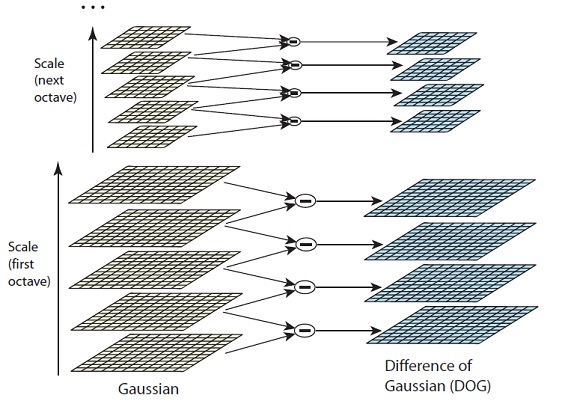
\includegraphics[width=0.90\textwidth]{fig/30.png}
     \vspace{-1em}
    \begin{center}    
       \caption{{\footnotesize \textit{(a) Nærliggende skalabilleder for hver oktav subtraheres og producere $DoG$ billederne. (b) I  $DoG$ billederne udvælges ekstremaer blandt 27 nabo pixels.}}}
    \label{fig:difference}
     \end{center}
     \vspace{-2.5em}
  \end{figure} \noindent    
Da $LoG$ svarer til, summen af hessian matricens egenværdier, vil et positivt filtersvar, angive et minima, hvor et negativt filtersvar vil angive et maxima, som angivet i ligning \eqref{laplaceblob}. Derfor identificeres ekstremaer i $DoG$ billederne, da de vil angive forekomster af blobs. For hver pixel, sammenlignes et $3\times3\times3$ område i $DoG$ billederne, som vist figur \ref{fig:difference} (b). Et punkt udvælges som værende et ekstrema, hvis det er den absolutte største værdi, iblandt dens 26 naboer.
\\
\\
Herefter anvender Lowe non-maximal surpression, som giver en nøjagtig placering af ekstremaer. \cite{nonmaximalsuppression}:
\begin{equation}
D(x)=D+\dfrac{\partial D^T}{\partial x}x\dfrac{1}{2}x^T\dfrac{\partial^2D}{\partial x^2}x
\label{nonmax}
\end{equation}
Ovenstående kan forstås om en Taylor udvidelse af punket D.
Placeringen af ekstremaet $\hat{x}$ findes ved at tage den afledte af den ovenstående funktion ift. $x$ og sætte den til 0:
\begin{equation}
\hat{x}= -\dfrac{\partial^2 D^{-1}}{\partial x^2}\dfrac{\partial D}{\partial x}
\label{xhat}
\end{equation}
Non-maximal surpression er i denne implementering anvendt anderledes end i SIFT: Lowe foreslår, at hvis et punkt er et ekstrema, som udregnet ved ligning \eqref{nonmax} og $\hat{x} > 0.5$ i en retning, skal ligning \eqref{nonmax} udregnes omkring det nye punkt og dette gentages, indtil $\hat{x} < 0.5$, eller indtil udregning er udført et max antal gange. I denne implementering er $\hat{x}$, brugt til at udvælge punkter, som er placeret på et ekstrema - dvs. hvis $|\hat{x}|$ > 0.5 i en given retning, er punktet ikke et interessepunkt.  Rationalet bag denne beslutning, vil blive diskuteret i afsnit 7.6.
\\
\\
Punkter med lav kontrast fjernes, ved at sætte grænseværdi, for $D(\hat{x})$:
\begin{equation}
D(\hat{x})=D+\dfrac{1}{2}\dfrac{\partial D^T}{\partial x}\hat{x}
\label{dxhat}
\end{equation}
Lowe foreslår at hvis $|D(\hat{x})|<0.03$ er punktet ikke et interessepunkt. \\ \\
$DoG$ returenere en stor værdi langs kanter. For at undgå at disse punkter udvælges som interessepunkter, anvendes en metode lånt fra Harris og Stephens \cite{harris}. Hessian matricen opstilles som:
\begin{equation}
\mathcal{H} =
\begin{bmatrix}
D_{xx} & D{xy} \\
D{xy} & D{yy}
\end{bmatrix}
\end{equation}
En negativ determinant angiver et saddel-punkt og fjernes. For at fjerne punkter lokaliseret på en kant beskrives forholdet imellem hessian matricens egenværdier, ved følgende ligning, hvor $r$ angiver størrelsesforholdet imellem egenværdierne:
\begin{equation}
\dfrac{tr(\mathcal{H})^2}{Det(\mathcal{H})}<\dfrac{(r+1)^2}{r}
\label{rval}
\end{equation}
En grænseværdi $r$ kan opstilles for at fjerne punkter lokaliseret på en kant. Punkter der tilfredsstiller denne grænseværdi udvælges som interessepunkter.
\subsubsection*{Algoritme: SIFT detektion}
\begin{tabbing}
Input\quad \= : \= Billede $I$\\
Output \text{ } \> : \> Interessepunkter $p \in (x,y)$
\end{tabbing}
\begin{enumerate}
\item{Skalarummet konstrueres for de forskellige oktaver, ved iterativt at folde skalabilledet med en stigende værdi af $\sigma$, hvor størrelsen af billedet halveres for hver oktav.}
\item{$DoG$ billederne udregnes,ved at subtrahere skalabillederne, som i ligning \eqref{dog}.}
\item{Ekstremaer lokaliseres for hvert punkt i $DoG$ billeder, ved at sammenligne punktet med dens 26 naboer som illustreret i figur \ref{fig:difference}.}
\item{Punkter der ikke er lokaliseret på ekstremaer, og ekstremaer med lav kontrast som i ligning \eqref{xhat} og \eqref{dxhat} afvises:
\begin{equation}
\begin{split}
\text{indikator} = 
\begin{cases}
\text{fjern}& \text{hvis } |\hat{x}|>0.5 \lor |D(\hat{x})|>0.03 \lor \bold{det} \mathcal{H}<0 , \\
\text{behold}& \text{ellers}. 
\end{cases}
\end{split}
\label{maxsurp}
\end{equation}
}
\item{Fjern punkter lokaliseret på en kant ved at opstille en grænseværdi $r$ og fjern punkter der ikke opfylder denne, som i ligning \eqref{rval}.}
\end{enumerate}